\chapter{Idea Progettuale: Modello degli Use Case e dei Processi}

In questo capitolo vengono presentati i principali use-case di \textit{Tuning Ledger}, la piattaforma per la gestione del \textit{Digital Modified Vehicle Passport} (DMVP), con l'obiettivo di descrivere in modo formale le interazioni tra gli attori e il sistema. Successivamente, i processi principali vengono modellati tramite diagrammi BPMN, al fine di rappresentare il flusso operativo delle attività di registrazione, esecuzione, certificazione e consegna del veicolo modificato.

\section{Modellazione degli Use-Case principali in GOREM}

La piattaforma, al fine di soddisfare tutte le richieste degli attori coinvolti, considera i casi d'uso di seguito riportati, organizzati per ciascuno degli stakeholder individuati nello scenario specifico. Coerentemente con la modellazione dei ruoli presentata nel Capitolo~3, a ogni ruolo corrisponde uno use-case: ciascuno stakeholder \textit{gioca} (\texttt{<<plays>>}) uno o più ruoli, e da ciascun ruolo discende l'operazione di cui esso è responsabile all'interno del sistema.

In tutti i diagrammi, le azioni che comportano una scrittura sul registro distribuito sono modellate come use-case inclusi (\texttt{<<include>>}) e vedono l'\textbf{Intermediario} come attore secondario, in quanto gestore della piattaforma e unico soggetto abilitato a operare sull'infrastruttura blockchain.

\subsection*{Concessionaria}

La Concessionaria gioca due ruoli, ai quali corrispondono altrettante operazioni (Figura~\ref{fig:uc-concessionaria}):

\begin{enumerate}
    \item \textit{Registrante del veicolo base}, che inserisce sulla piattaforma i dati identificativi del veicolo originale forniti dalla Casa Automobilistica e le modifiche commissionate dal Cliente Privato. L'operazione include l'inizializzazione del DMVP, ossia la creazione dell'istanza del passaporto digitale associata univocamente al numero di telaio.
    \item \textit{Responsabile della consegna}, che avvia la procedura di consegna del veicolo omologato al termine dell'iter tecnico. L'operazione include la registrazione della consegna sul DMVP.
\end{enumerate}

\begin{figure}[H]
    \centering
    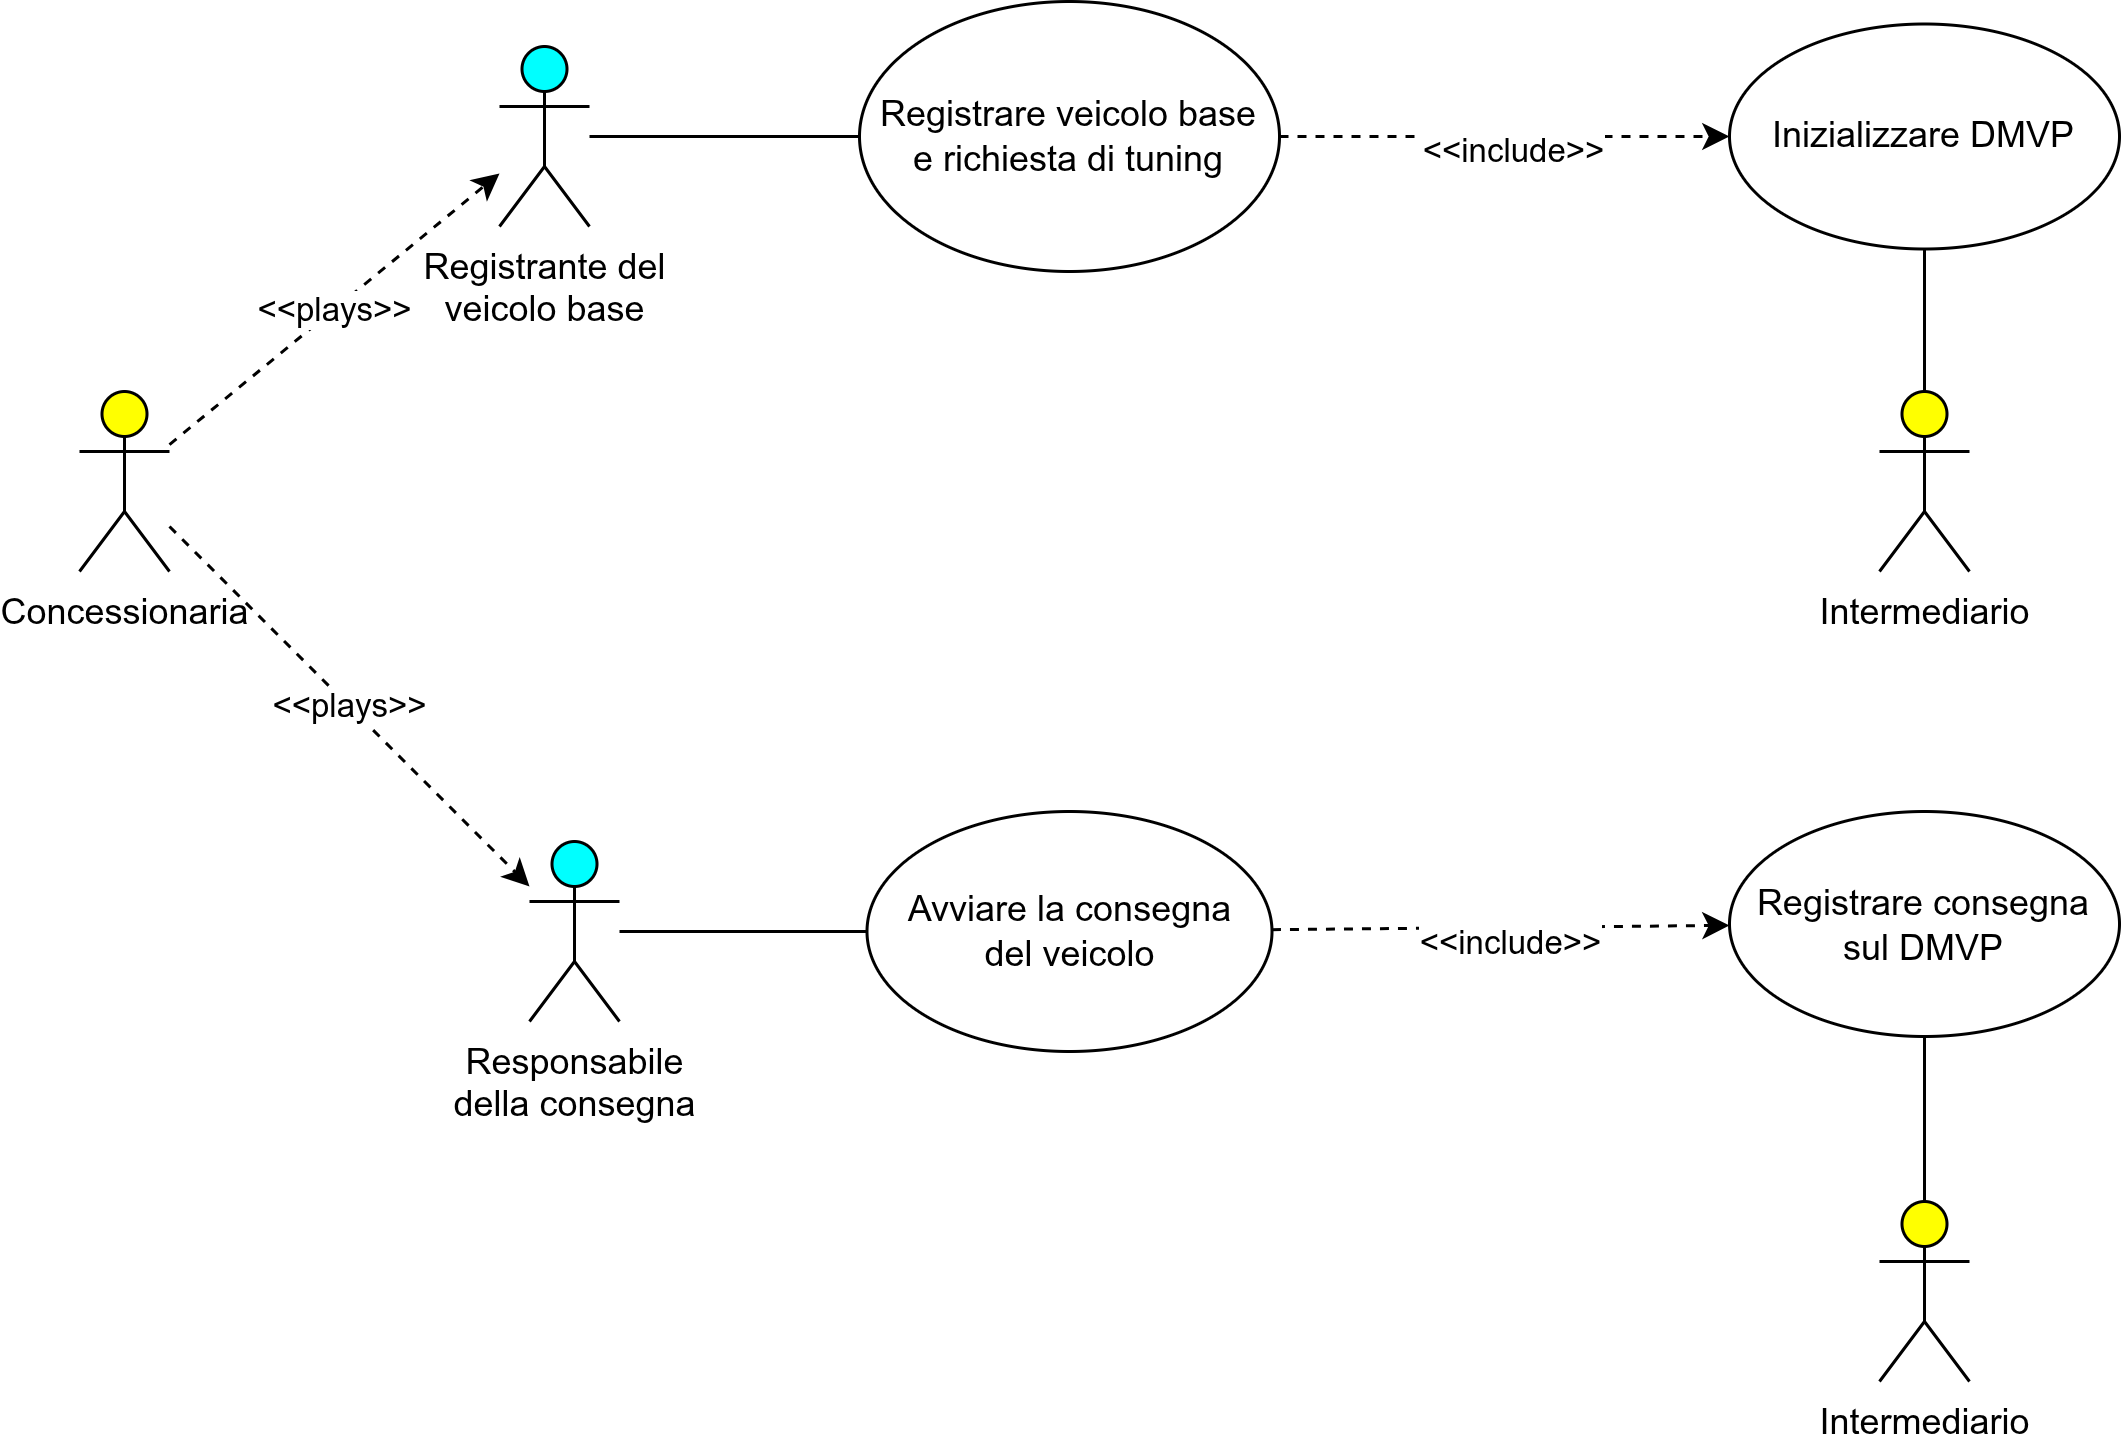
\includegraphics[width=\textwidth]{imgs/usecase/01_concessionaria.png}
    \caption{Use-Case Concessionaria}
    \label{fig:uc-concessionaria}
\end{figure}

\subsection*{Azienda di Tuning}

L'Azienda di Tuning gioca il ruolo di \textit{Esecutore delle modifiche}, responsabile della registrazione sul DMVP delle lavorazioni effettivamente eseguite sul veicolo. Tale operazione si articola in tre azioni incluse (Figura~\ref{fig:uc-tuning}):

\begin{itemize}
    \item la compilazione della \textbf{scheda tecnica modificata}, contenente le specifiche degli interventi e i codici seriali dei componenti installati;
    \item l'acquisizione delle \textbf{prove multimediali} a corredo delle lavorazioni, quali fotografie e documentazione tecnica;
    \item l'\textbf{ancoraggio dell'hash} dei dati registrati sulla blockchain, eseguito tramite l'Intermediario.
\end{itemize}

Quest'ultimo punto rende esplicita l'architettura ibrida della soluzione: la documentazione voluminosa risiede nel database off-chain, mentre sulla catena viene registrata soltanto l'impronta crittografica che ne garantisce l'integrità.

\begin{figure}[H]
    \centering
    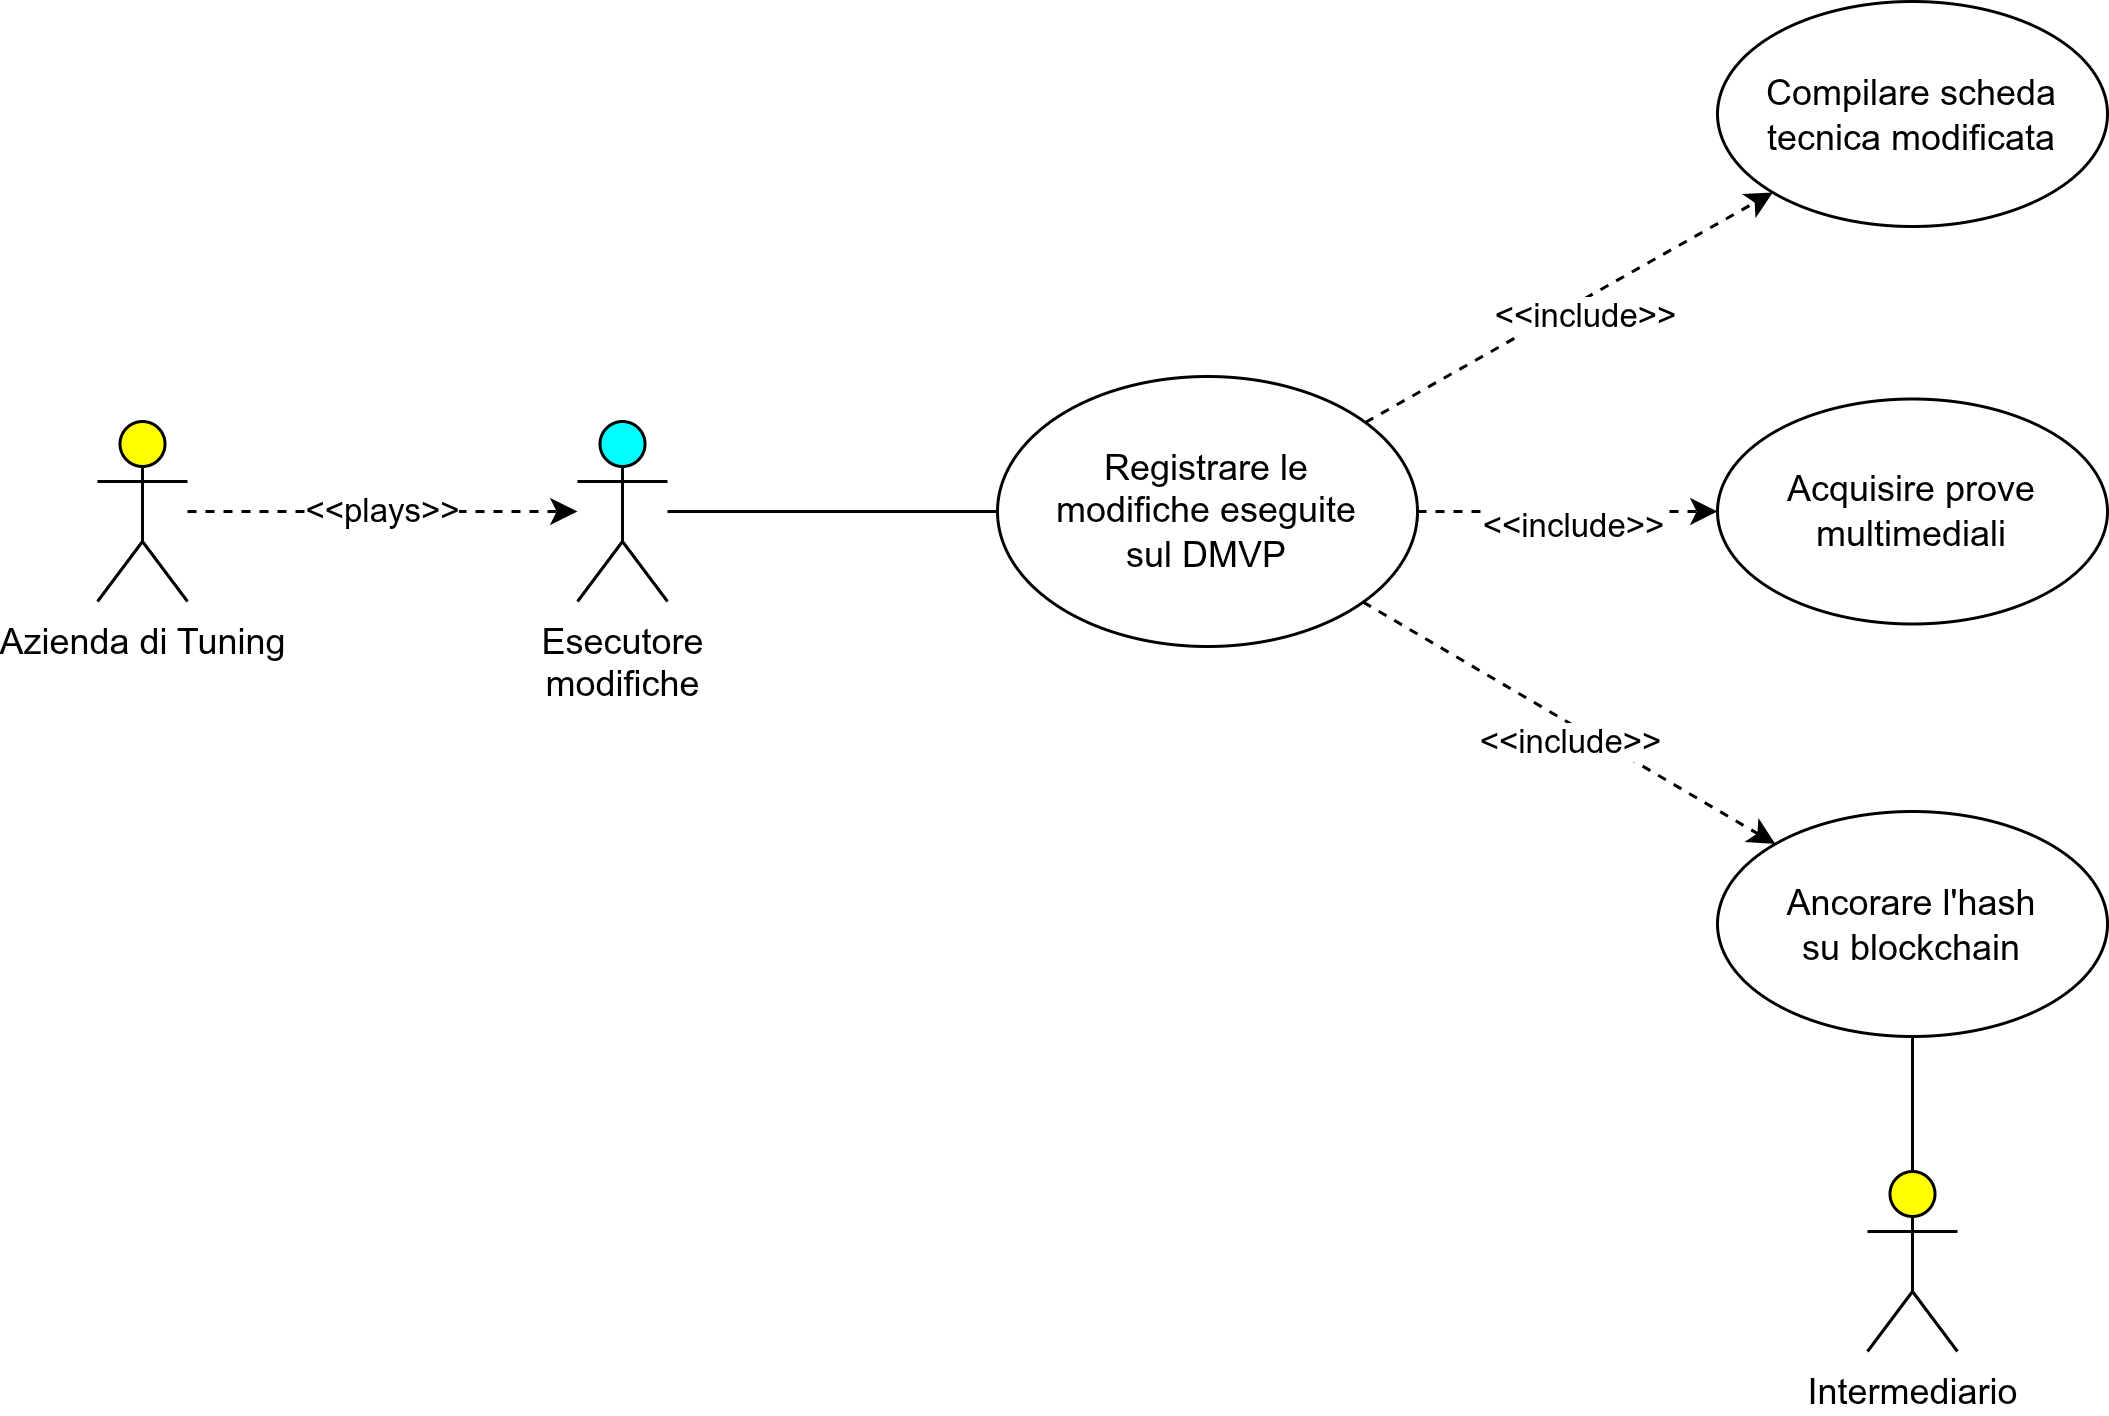
\includegraphics[width=\textwidth]{imgs/usecase/02_azienda_di_tuning.png}
    \caption{Use-Case Azienda di Tuning}
    \label{fig:uc-tuning}
\end{figure}

\subsection*{Centro di Certificazione}

Il Centro di Certificazione gioca due ruoli distinti (Figura~\ref{fig:uc-certificazione}), corrispondenti alle due fasi logicamente separate della sua attività:

\begin{enumerate}
    \item \textit{Ispettore/Collaudatore}, che esegue le verifiche tecniche e normative sulle modifiche apportate. L'operazione include la consultazione dello storico del DMVP, necessaria per accertare che tutte le fasi precedenti siano state svolte correttamente. A tale use-case è associata, come flusso alternativo, la \textbf{segnalazione di non conformità} (\texttt{<<extend>>}), attivata nel caso in cui il collaudo dia esito negativo.
    \item \textit{Emittente della certificazione}, che rilascia il certificato digitale di conformità al superamento del collaudo. L'operazione include la registrazione del certificato sulla blockchain, con conseguente aggiornamento dello stato del DMVP.
\end{enumerate}

\begin{figure}[H]
    \centering
    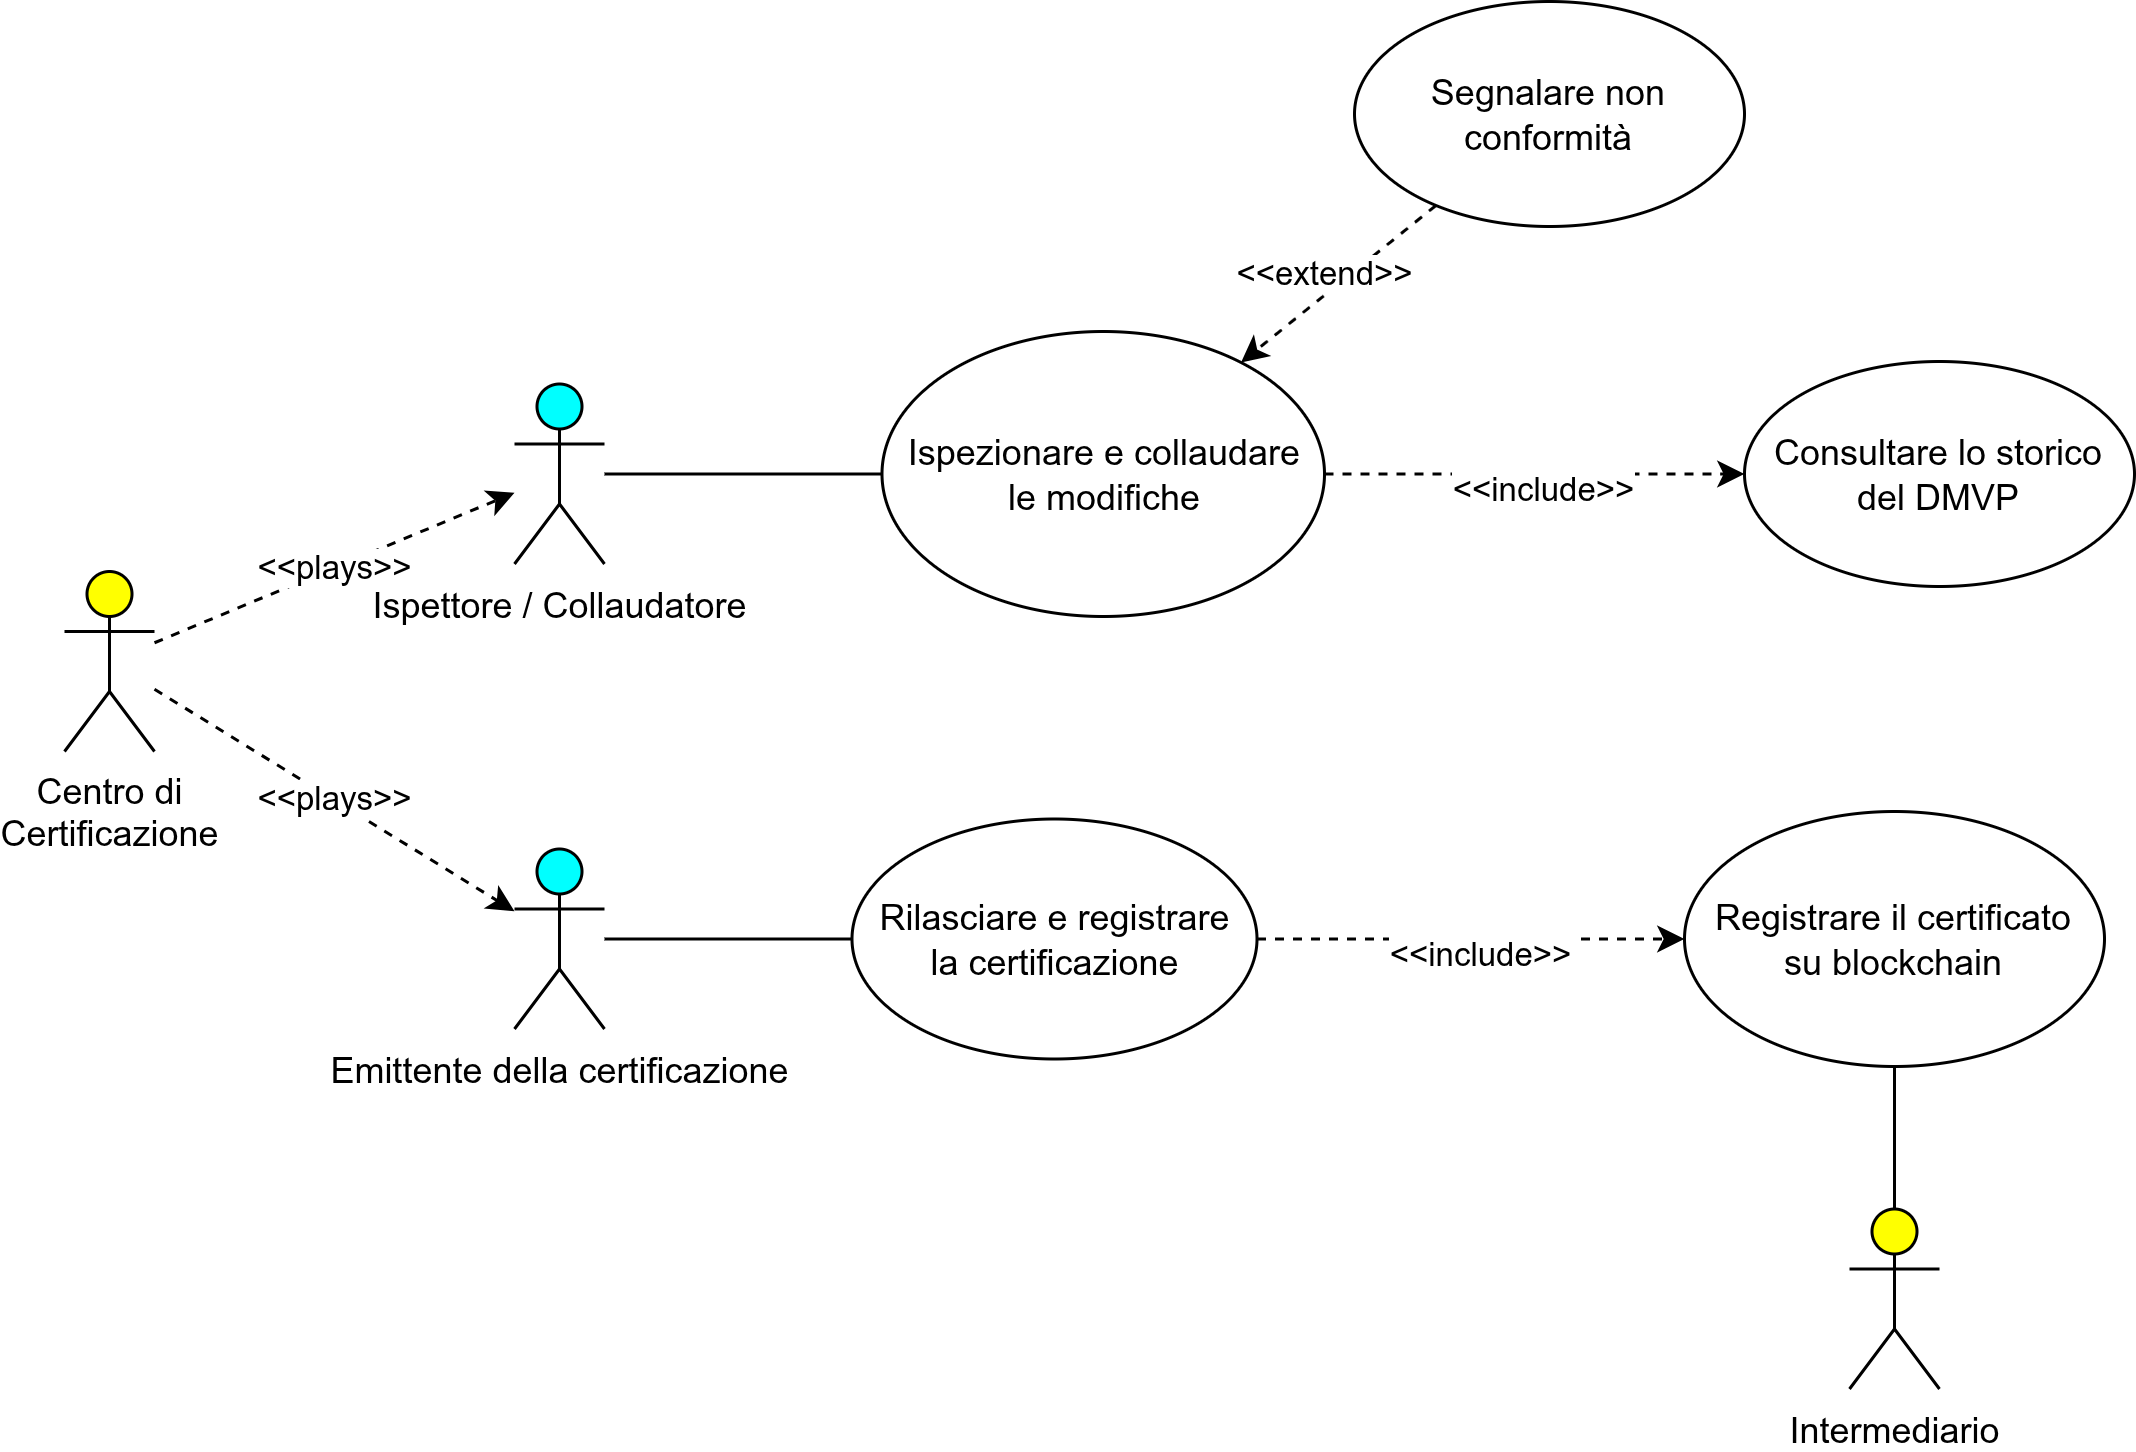
\includegraphics[width=\textwidth]{imgs/usecase/03_centro_di_certificazione.png}
    \caption{Use-Case Centro di Certificazione}
    \label{fig:uc-certificazione}
\end{figure}

\subsection*{Cliente Privato}

Il Cliente Privato gioca due ruoli (Figura~\ref{fig:uc-cliente}):

\begin{enumerate}
    \item \textit{Consultatore dello storico}, che accede in sola lettura al registro immutabile del veicolo per verificarne l'autenticità e ricostruirne la storia completa, sia prima dell'accettazione sia in qualunque momento successivo.
    \item \textit{Acquirente/nuovo proprietario}, che accetta il veicolo al termine della consegna e ne riceve il passaporto digitale. L'operazione include il trasferimento della proprietà del DMVP, registrato sulla blockchain tramite l'Intermediario.
\end{enumerate}

\begin{figure}[H]
    \centering
    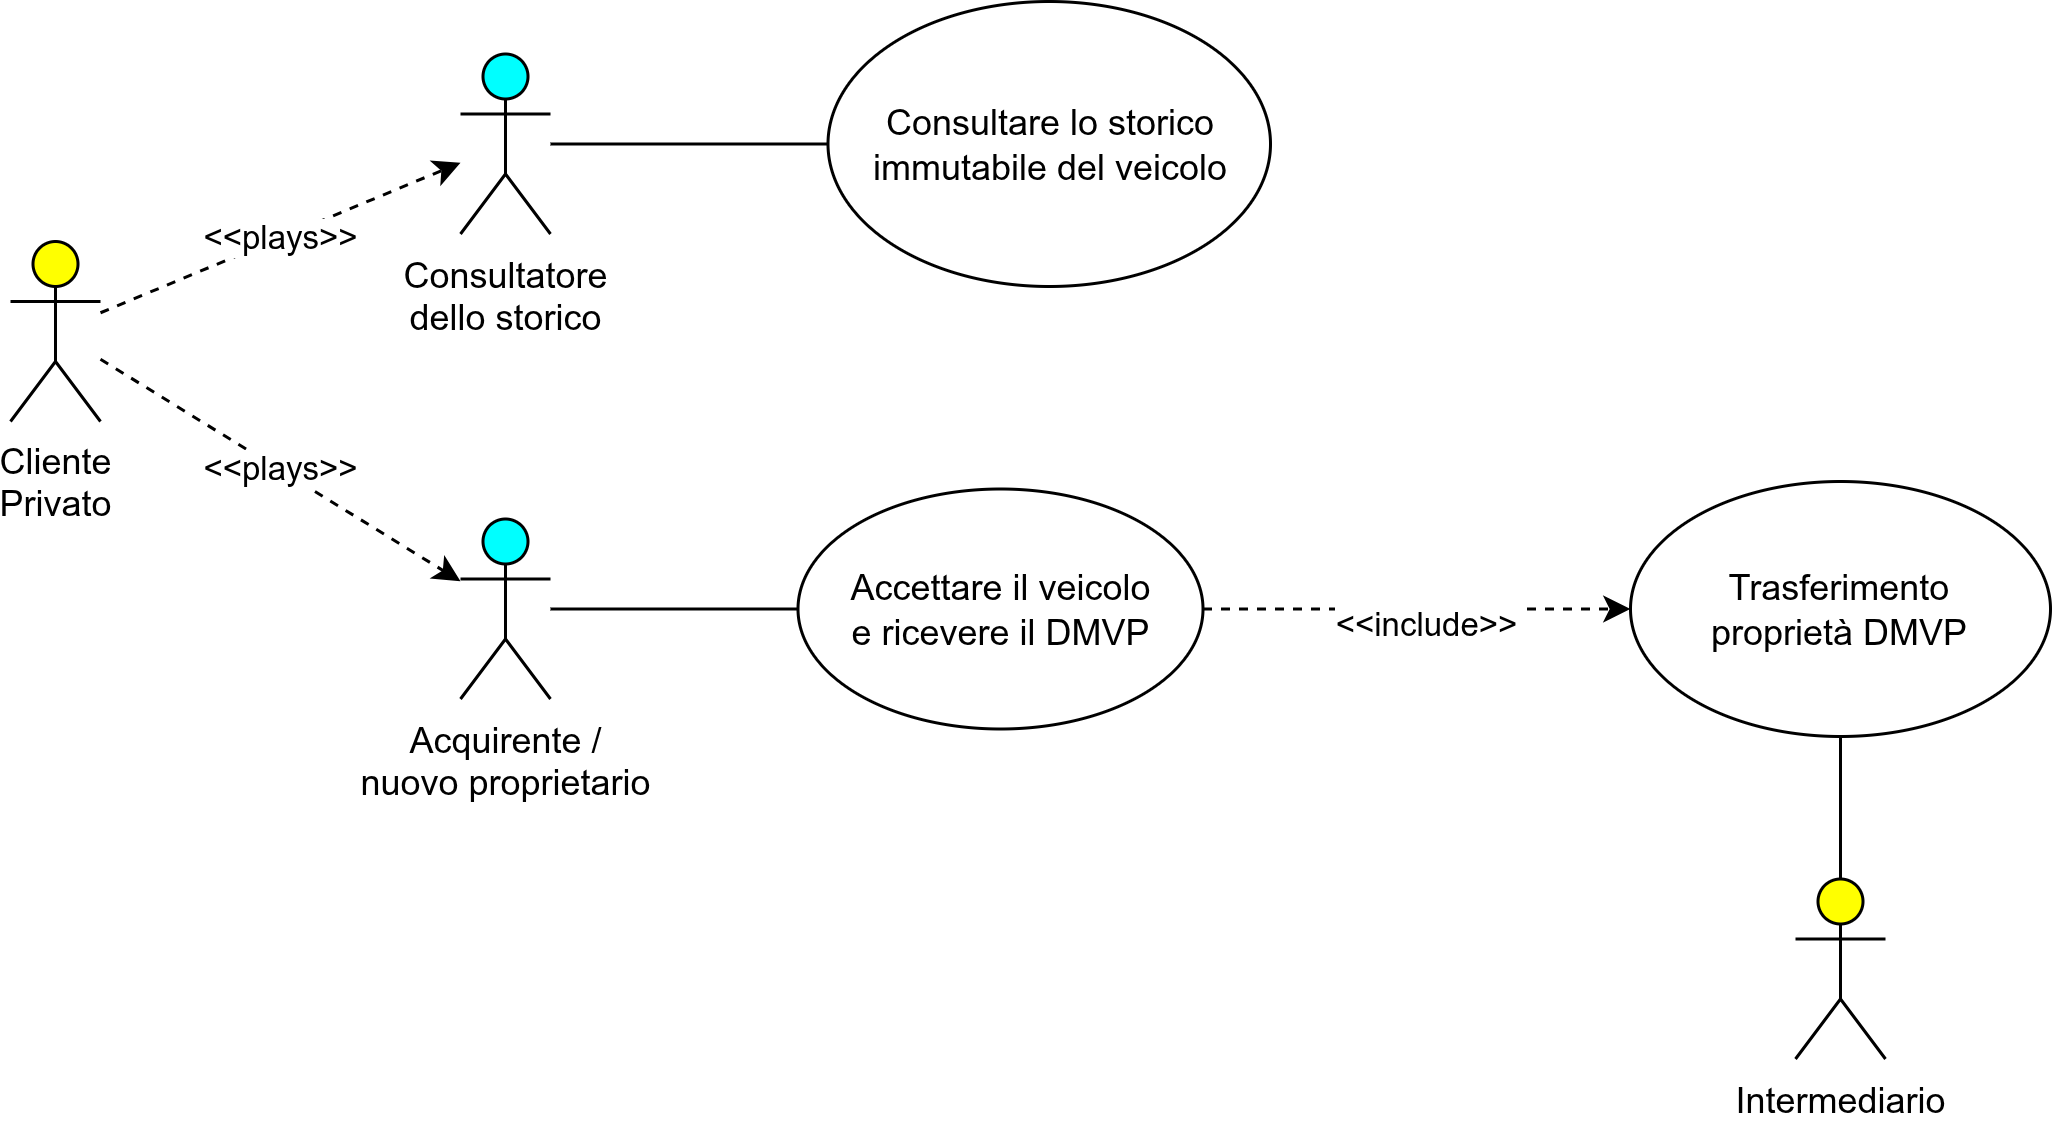
\includegraphics[width=\textwidth]{imgs/usecase/04_cliente_privato.png}
    \caption{Use-Case Cliente Privato}
    \label{fig:uc-cliente}
\end{figure}

\subsection*{Intermediario}

L'Intermediario, in qualità di gestore della piattaforma, gioca tre ruoli (Figura~\ref{fig:uc-intermediario}):

\begin{enumerate}
    \item \textit{Amministratore della piattaforma}, che configura e mantiene l'infrastruttura blockchain permissioned, definendo i canali, le politiche di \textit{endorsement} e i parametri di funzionamento della rete.
    \item \textit{Gestore delle identità e onboarding}, che registra e verifica le identità degli attori ammessi alla rete, emettendo le credenziali necessarie all'operatività sulla piattaforma. Si tratta del presupposto di affidabilità dell'intero sistema: soltanto soggetti verificati possono scrivere sul registro.
    \item \textit{Assistente all'uso della piattaforma}, che fornisce supporto operativo e formativo a tutti gli altri stakeholder. Tale use-case è infatti invocato da Concessionaria, Azienda di Tuning, Centro di Certificazione e Cliente Privato.
\end{enumerate}

\begin{figure}[H]
    \centering
    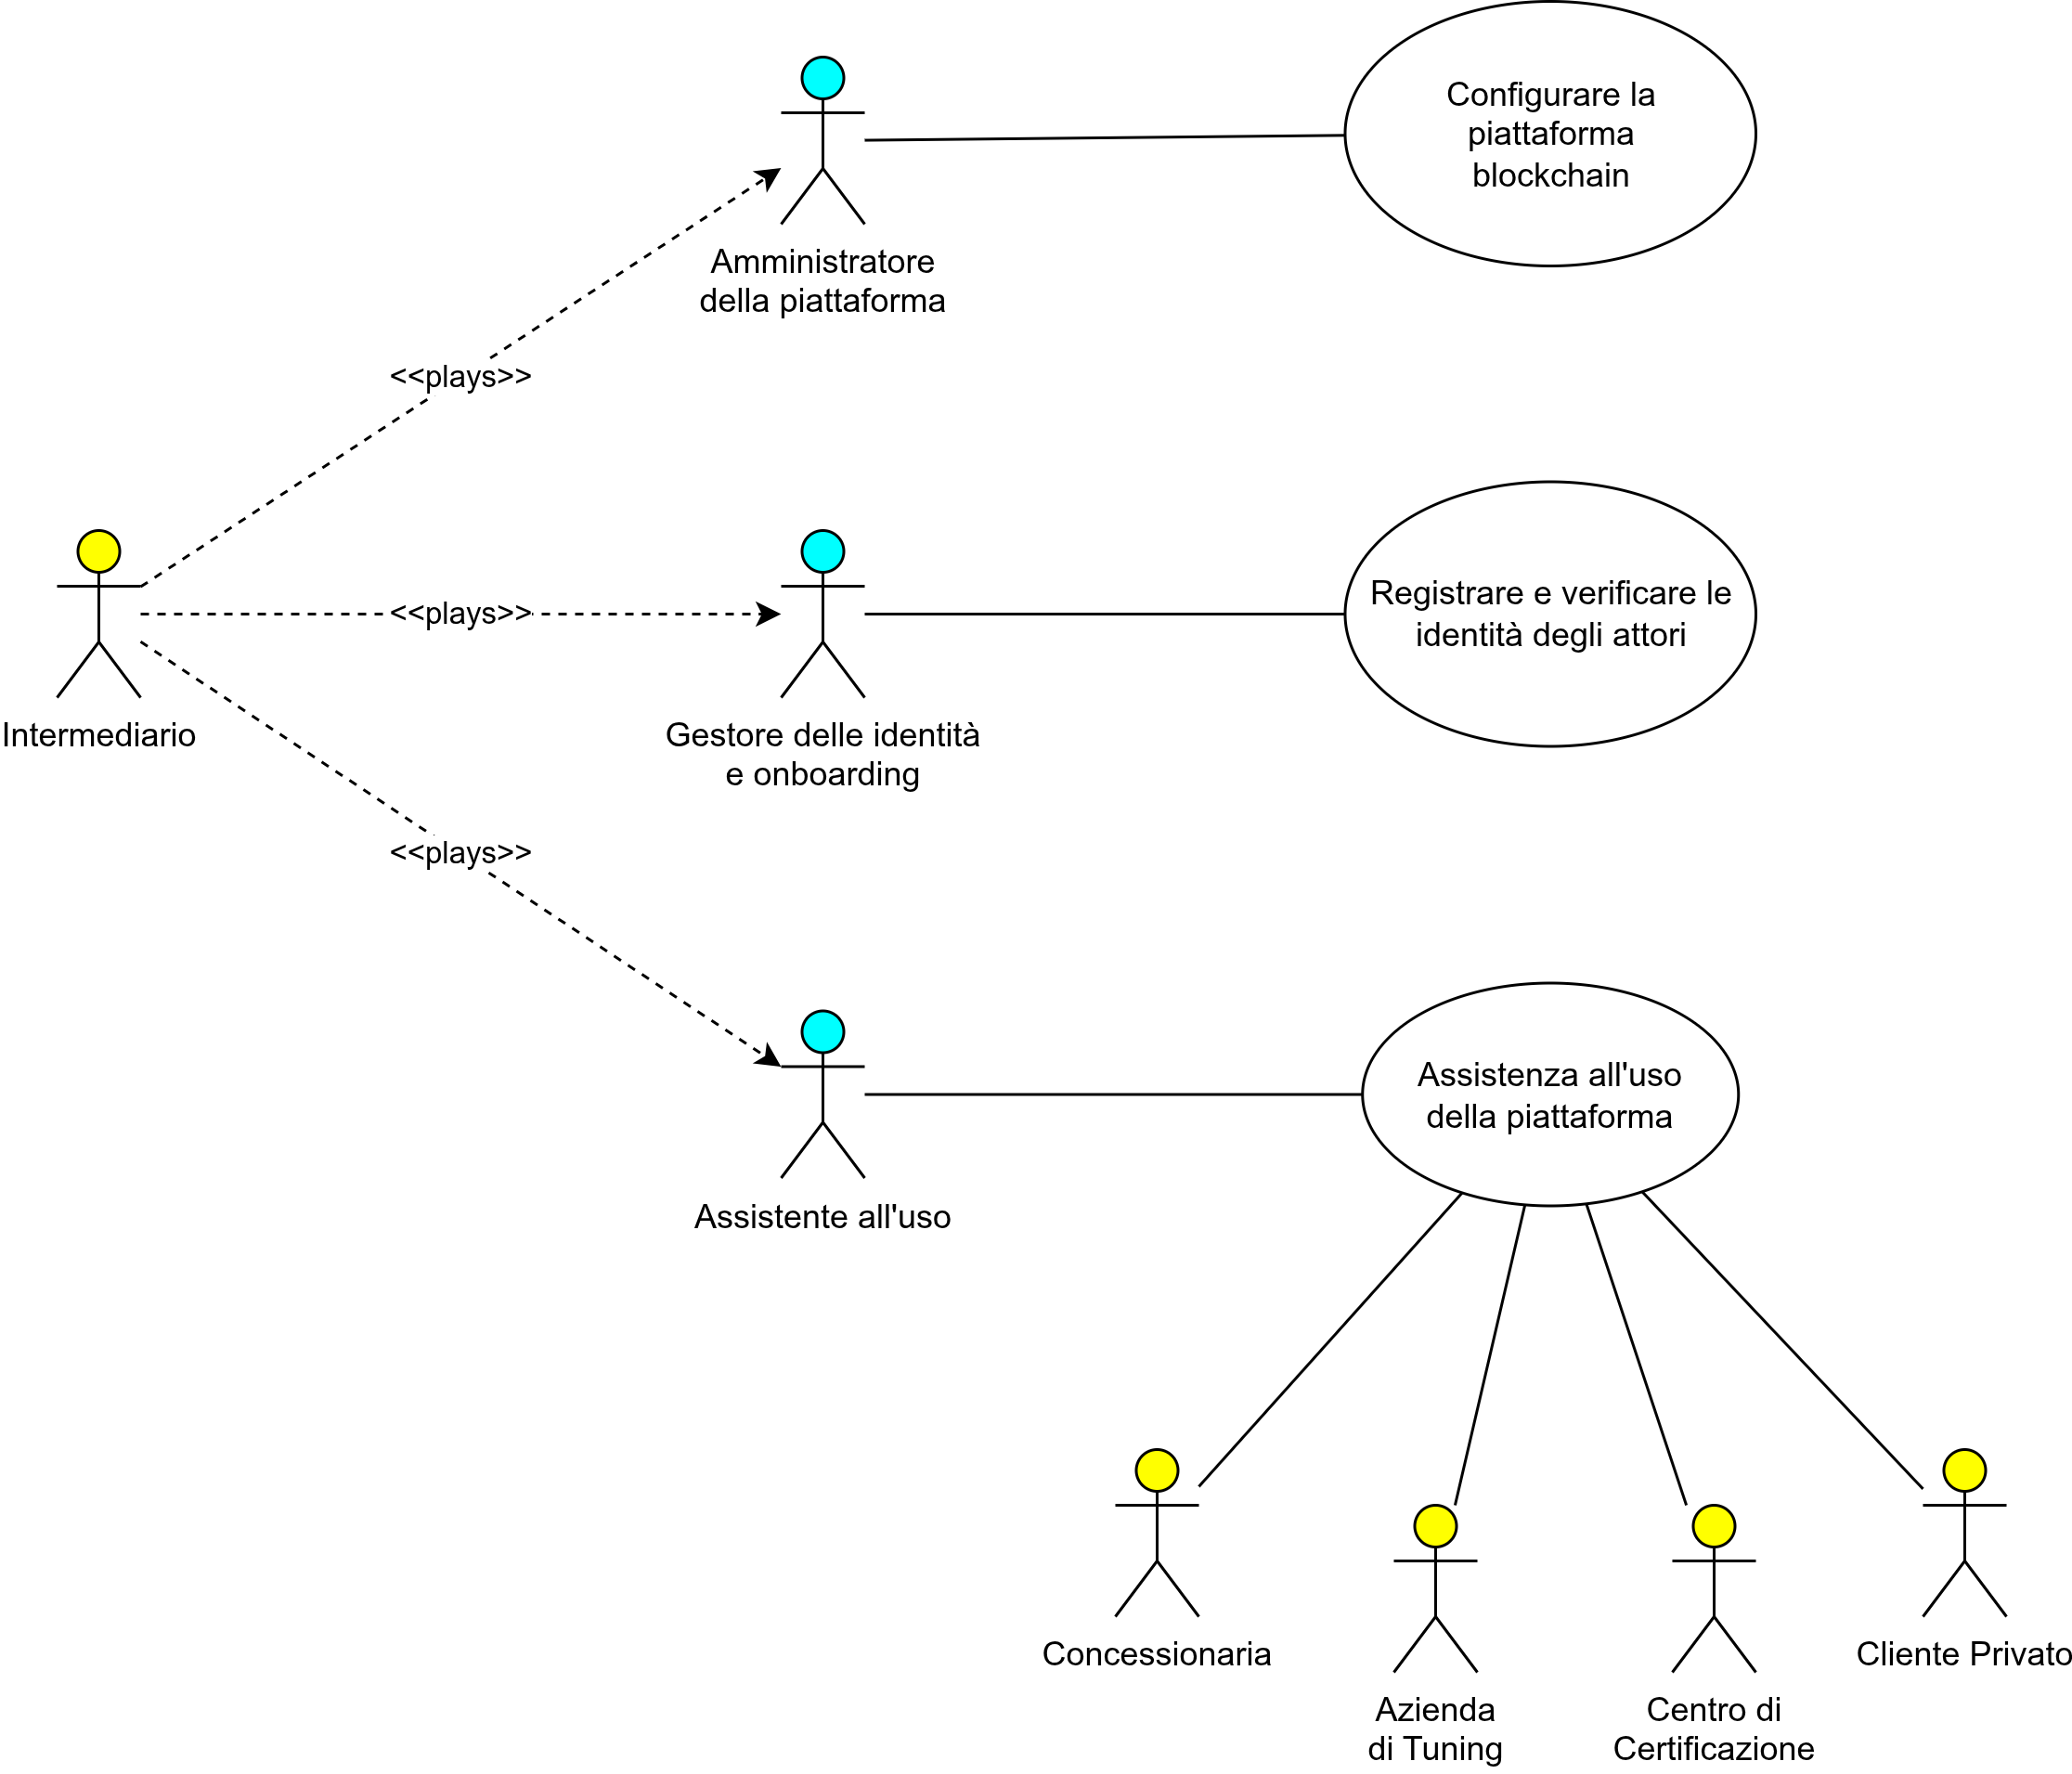
\includegraphics[width=\textwidth]{imgs/usecase/05_intermediario.png}
    \caption{Use-Case Intermediario}
    \label{fig:uc-intermediario}
\end{figure}

\section{Modellazione dei Processi principali in BPMN}

A valle della rappresentazione dei casi d'uso, è importante illustrare quali siano i processi fondamentali che avvengono all'interno della filiera in esame. A tal fine viene sfruttato il formalismo \textbf{BPMN} (\textit{Business Process Model and Notation}), rappresentazione grafica utilizzata per modellare e descrivere i processi aziendali. I diagrammi illustrano una coreografia, in cui ogni attività è svolta da un partecipante e indirizzata a uno o più altri partecipanti.

La modellazione dei processi ha l'obiettivo di:

\begin{itemize}
    \item rendere esplicite le responsabilità dei diversi attori coinvolti;
    \item descrivere il flusso informativo e decisionale lungo il ciclo di vita del veicolo modificato;
    \item evidenziare le interazioni tra la componente off-chain e l'infrastruttura blockchain;
    \item garantire la coerenza tra requisiti funzionali, casi d'uso e scelte tecnologiche.
\end{itemize}

In tutti i diagrammi la piattaforma, rappresentata dall'\textbf{Intermediario} e dall'infrastruttura blockchain sottostante, opera come componente di supporto trasversale, garantendo immutabilità dei dati, validazione delle informazioni e tracciabilità temporale delle operazioni. I due archivi di dati sono rappresentati distintamente: l'\textit{Off-Chain Database}, che conserva i dati descrittivi e i documenti, e la \textit{Blockchain}, sulla quale viene ancorata la sola impronta crittografica.

\subsection*{Processo Complessivo di Gestione del DMVP}

La Figura~\ref{fig:bpmn-complessivo} illustra l'architettura macroscopica del processo collaborativo, che descrive l'intero ciclo di vita del passaporto digitale dalla registrazione iniziale del veicolo fino al trasferimento finale della proprietà al cliente.

\begin{figure}[H]
    \centering
    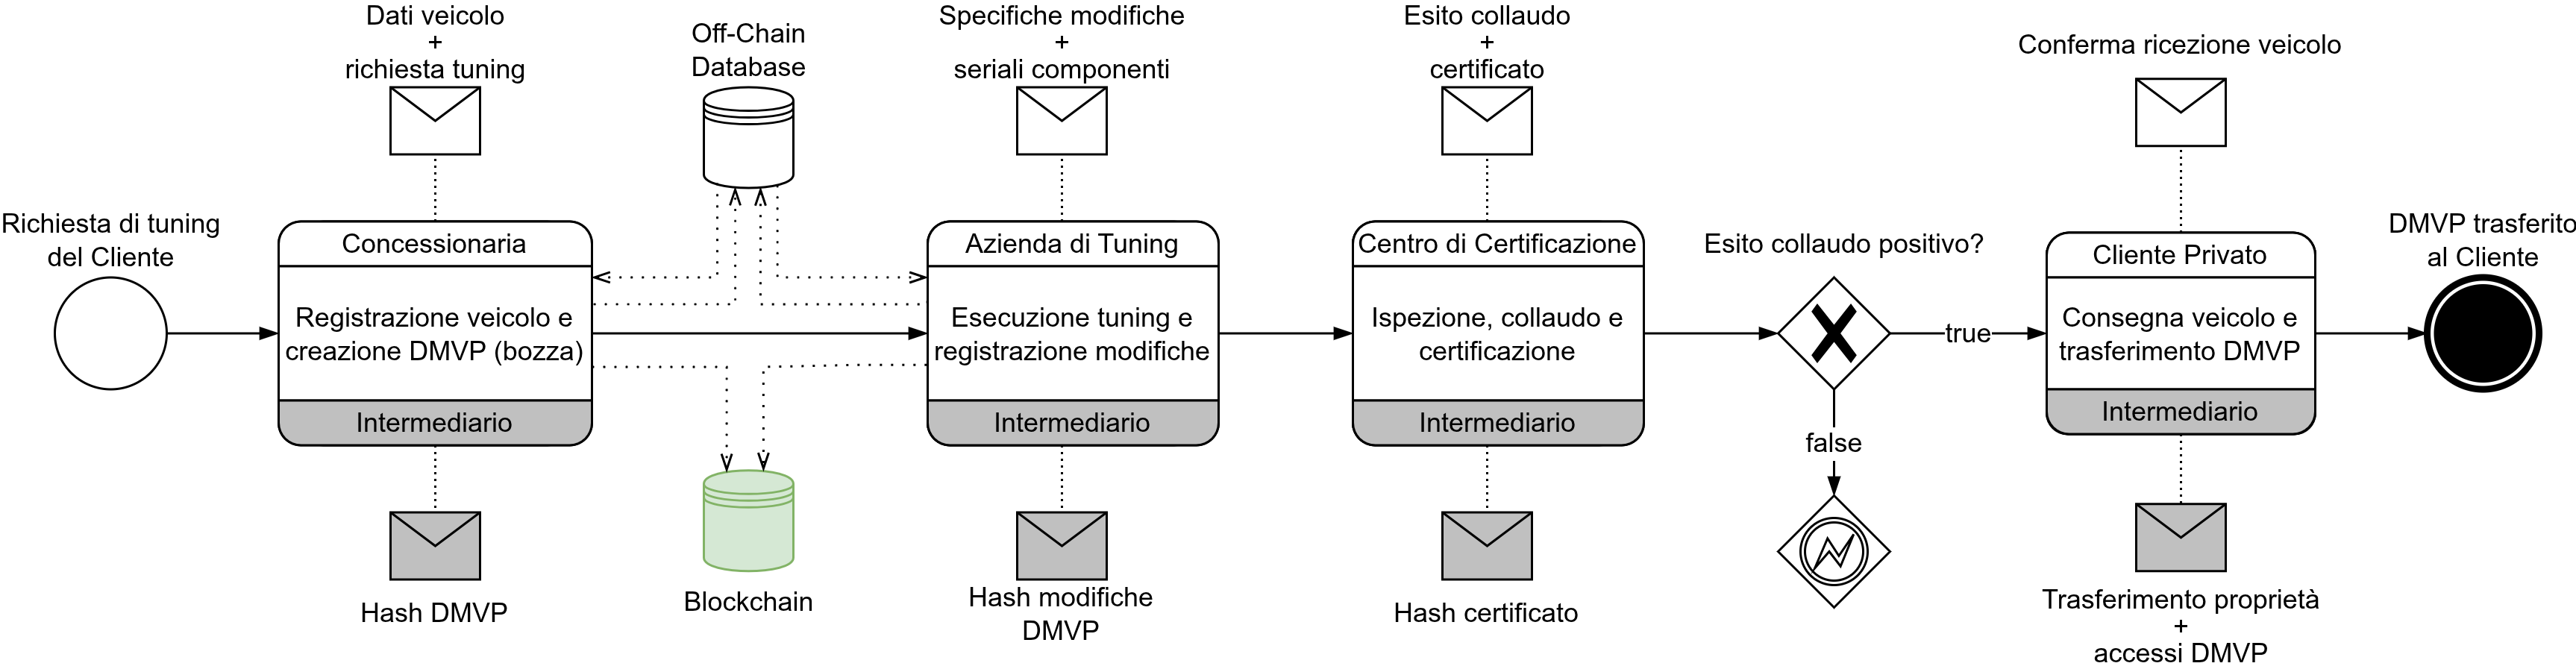
\includegraphics[width=\textwidth]{imgs/bpmn/00_gestione_DMVP.png}
    \caption{Processo complessivo di gestione del DMVP}
    \label{fig:bpmn-complessivo}
\end{figure}

Il flusso ha un andamento sequenziale e può essere idealmente suddiviso in quattro macro-fasi:

\begin{enumerate}
    \item \textbf{Registrazione del veicolo e creazione del DMVP}: l'innesco del processo avviene con la richiesta di tuning formulata dal Cliente Privato. La Concessionaria registra il veicolo base e genera una prima istanza del DMVP in stato di bozza, il cui hash viene ancorato sulla catena.
    \item \textbf{Esecuzione del tuning e registrazione delle modifiche}: l'Azienda di Tuning esegue le lavorazioni e ne registra le specifiche tecniche insieme ai seriali dei componenti installati, ancorando l'hash delle modifiche al DMVP.
    \item \textbf{Ispezione, collaudo e certificazione}: il Centro di Certificazione verifica la conformità tecnica e normativa degli interventi. Un \textit{Gateway Esclusivo} discrimina l'esito del collaudo: in caso negativo il processo termina con un evento di eccezione che rimanda le lavorazioni all'Azienda di Tuning; in caso positivo viene emesso il certificato digitale e il relativo hash viene registrato sulla catena.
    \item \textbf{Consegna e trasferimento}: il processo si conclude con la consegna del veicolo omologato e il trasferimento definitivo della proprietà e dei diritti di accesso al DMVP all'account del Cliente Privato.
\end{enumerate}

Al fine di garantire l'autenticità e l'affidabilità delle informazioni, ogni trasferimento di responsabilità o cambio di stato rilevante tra i soggetti della filiera viene ancorato in maniera indelebile sulla blockchain. Di seguito vengono analizzati i quattro sotto-processi di dettaglio.

\subsection*{Processo di Registrazione del Veicolo e Richiesta di Tuning}

Questo processo modella la fase di inizializzazione del passaporto digitale. Il flusso ha inizio nel momento in cui il Cliente Privato formalizza l'acquisto del veicolo e richiede una personalizzazione presso la Concessionaria, che avvia la procedura sulla piattaforma.

All'interno del diagramma di Figura~\ref{fig:bpmn-registrazione}, la Concessionaria inserisce i dati identificativi del veicolo e le modifiche richieste; la piattaforma esegue quindi una verifica di completezza dei dati, modellata come sotto-processo. Un \textbf{Gateway Esclusivo (XOR)} discrimina tra dati validi e dati incompleti: in caso di esito negativo il flusso viene reindirizzato, tramite un gateway di merge, all'attività di inserimento, richiedendo una nuova compilazione.

In caso di esito positivo, il processo prevede l'attivazione dell'Intermediario, che salva i dati descrittivi nel database off-chain e genera una prima transazione su blockchain per ancorare temporalmente la richiesta. Il processo si conclude con la notifica di presa in carico inviata all'Azienda di Tuning.

\begin{figure}[H]
    \centering
    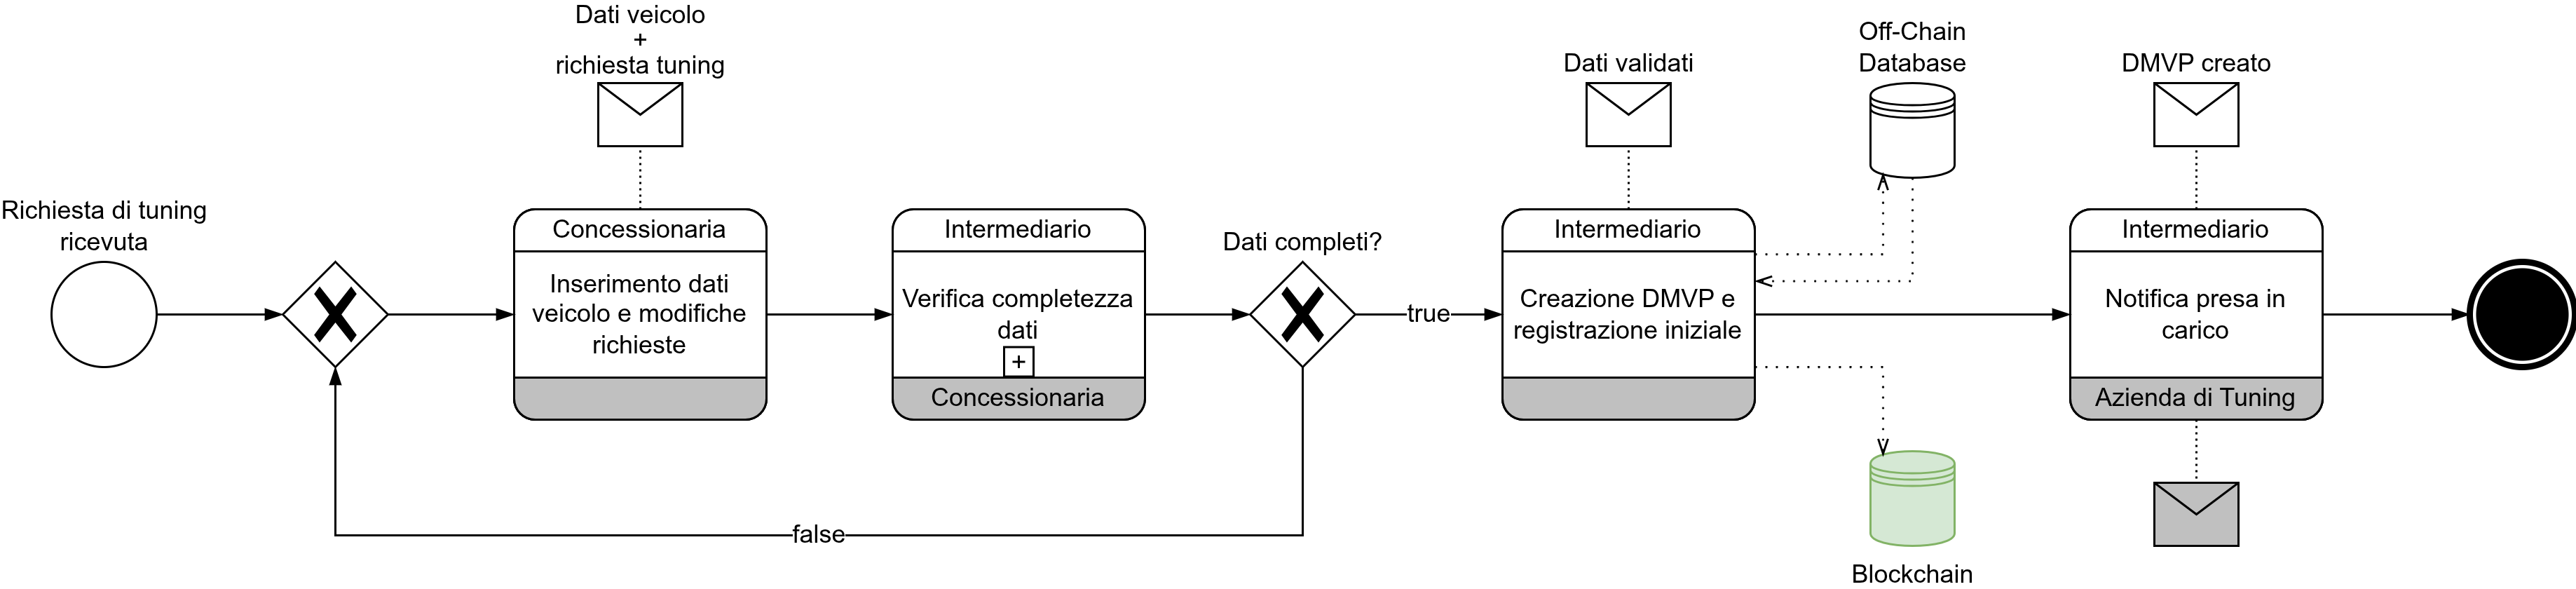
\includegraphics[width=\textwidth]{imgs/bpmn/01_registrazione_veicolo_e_richiesta_tuning.png}
    \caption{Processo di registrazione del veicolo e richiesta di tuning}
    \label{fig:bpmn-registrazione}
\end{figure}

\subsection*{Processo di Esecuzione del Tuning e Registrazione delle Modifiche}

Il diagramma di Figura~\ref{fig:bpmn-tuning} rappresenta il cuore operativo della piattaforma, descrivendo la fase di personalizzazione del veicolo. Il processo è attivato dalla ricezione della richiesta di lavorazione da parte dell'Azienda di Tuning.

Il flusso si articola in due macro-attività eseguite in parallelo, modellate tramite un \textbf{Gateway Parallelo (AND)}: l'esecuzione fisica delle modifiche sul veicolo, rappresentata come sotto-processo, e la rendicontazione digitale delle lavorazioni effettuate. In quest'ultima l'Azienda di Tuning inserisce le specifiche tecniche degli interventi, i codici seriali dei componenti installati e la documentazione tecnica associata.

La piattaforma provvede quindi al salvataggio strutturato delle informazioni nel database off-chain e alla registrazione del relativo hash sulla blockchain, garantendo l'immutabilità e la tracciabilità delle modifiche. I due rami convergono in un gateway di sincronizzazione e il processo si conclude con l'invio automatico di una notifica al Centro di Certificazione, che avvia la fase di collaudo.

\begin{figure}[H]
    \centering
    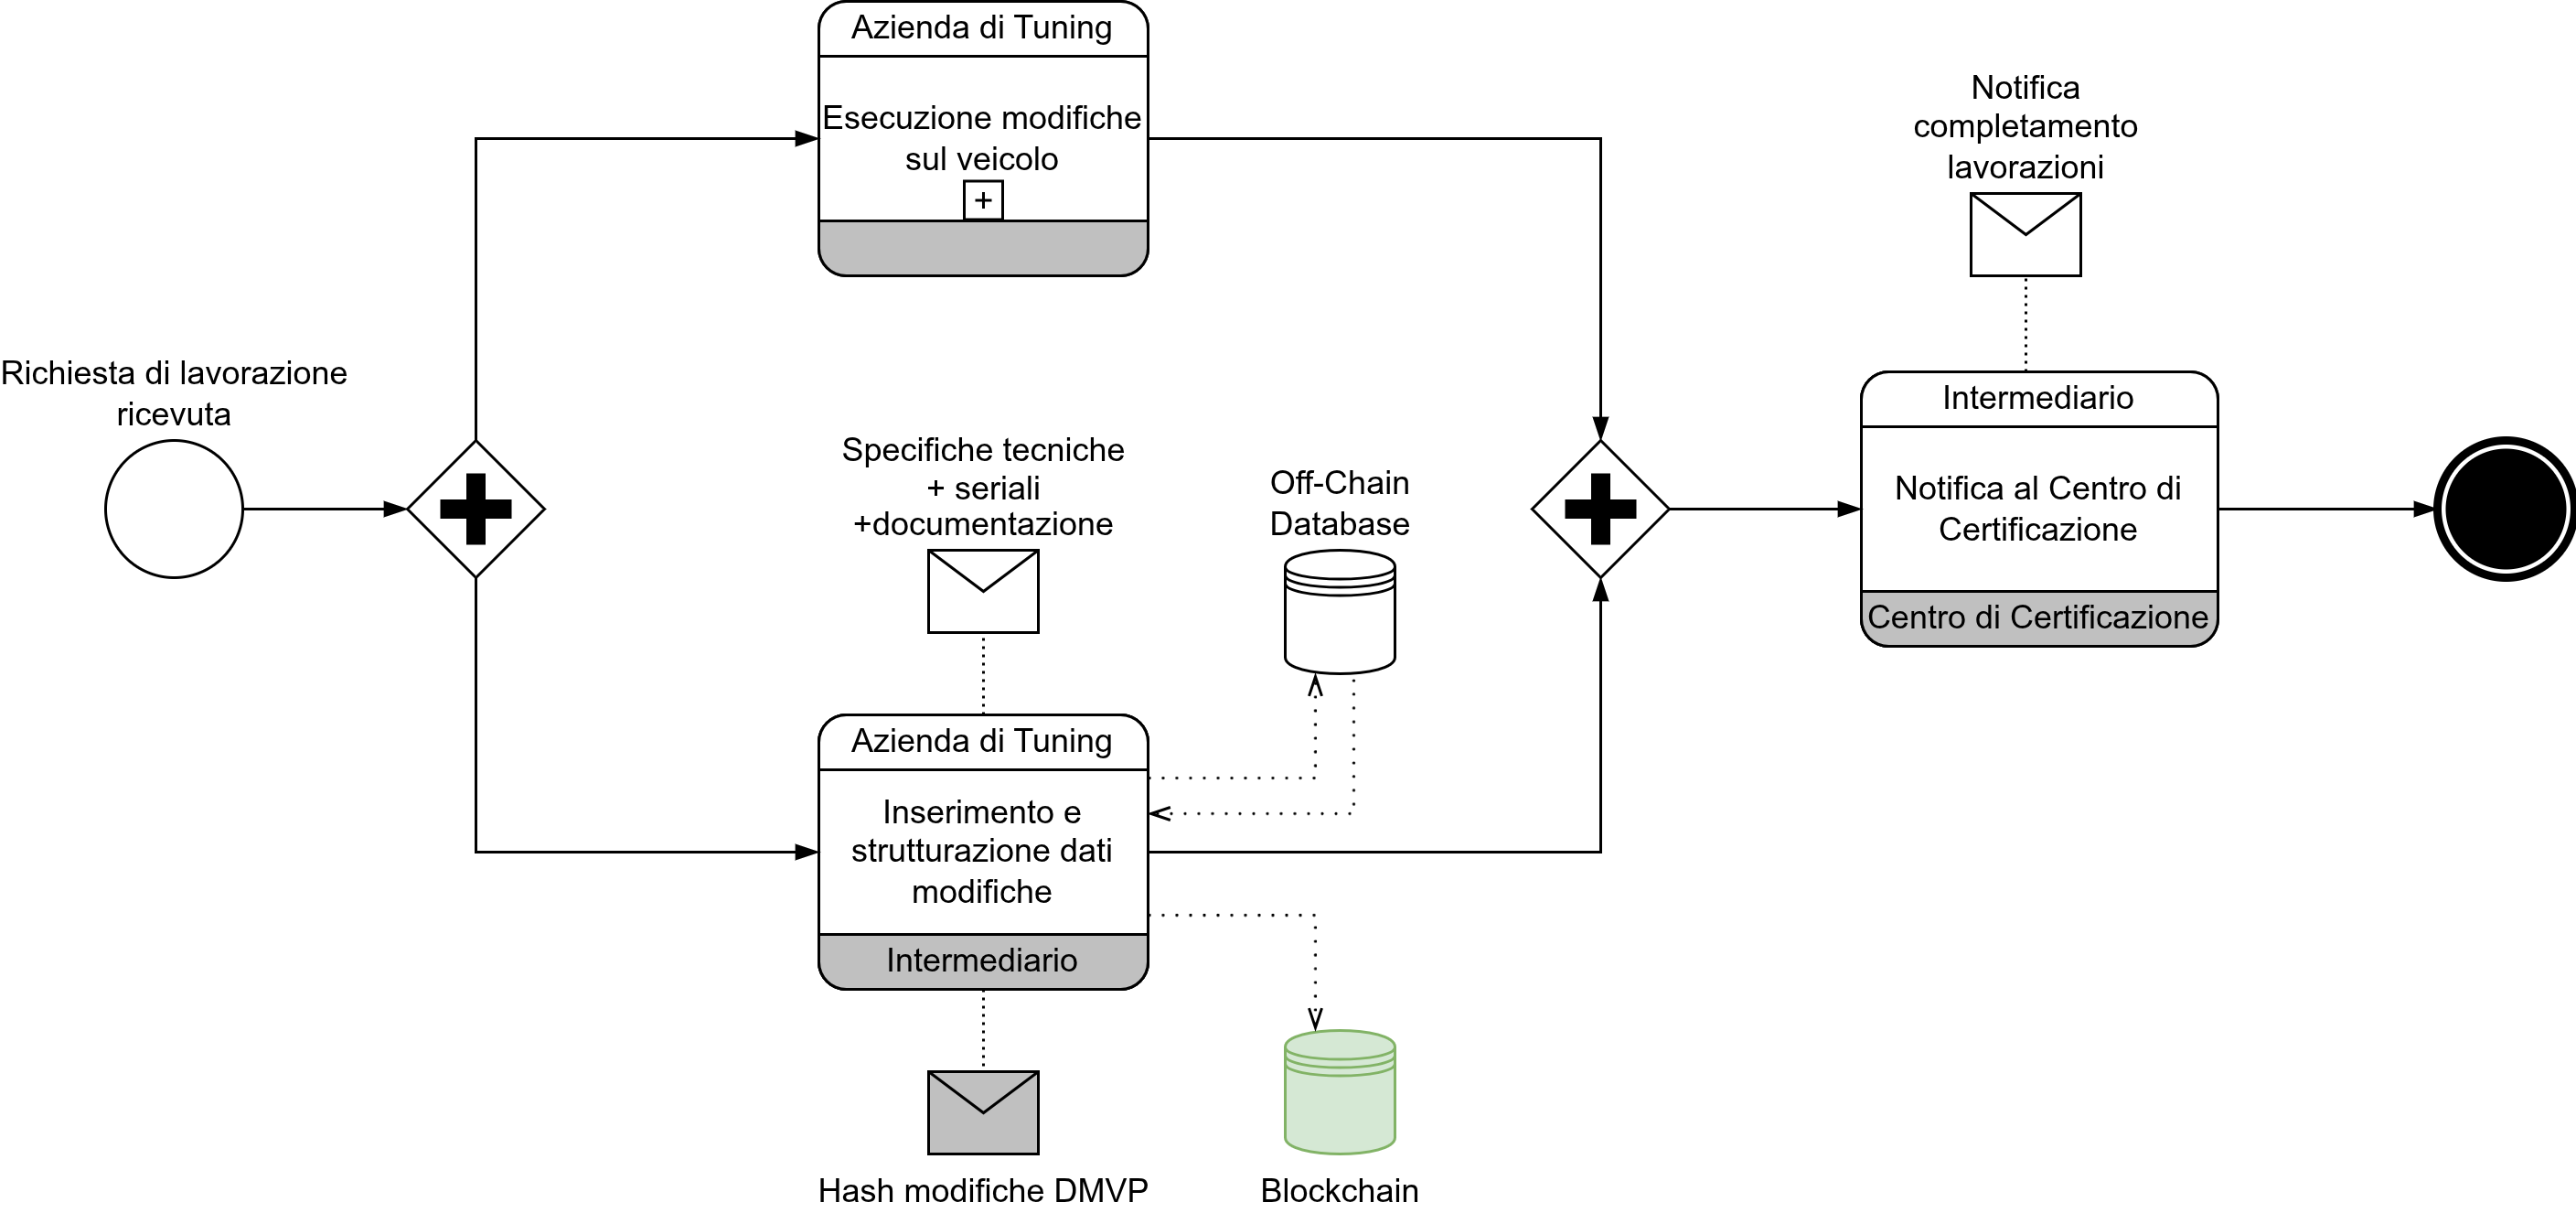
\includegraphics[width=\textwidth]{imgs/bpmn/02_esecuzione_tuning_e_registrazione_modifiche.png}
    \caption{Processo di esecuzione del tuning e registrazione delle modifiche}
    \label{fig:bpmn-tuning}
\end{figure}

\subsection*{Processo di Ispezione e Certificazione}

Il terzo processo (Figura~\ref{fig:bpmn-certificazione}) formalizza la fase di ispezione tecnica e certificazione normativa. Il flusso ha inizio con la presa in carico del veicolo da parte del Centro di Certificazione, che consulta i dati storici del DMVP registrati sulla piattaforma ed esegue le verifiche tecniche e normative previste, modellate come sotto-processo.

Un \textbf{Gateway Esclusivo (XOR)} gestisce l'esito dell'ispezione:

\begin{itemize}
    \item \textbf{Caso negativo}: le modifiche risultano non conformi. Viene generato un report di anomalia e il ramo termina con un \textit{Message End Event} indirizzato all'Azienda di Tuning, alla quale la pratica viene reindirizzata per le necessarie correzioni.
    \item \textbf{Caso positivo}: il collaudo è superato e viene emesso il certificato digitale.
\end{itemize}

In caso di esito positivo il certificato viene archiviato nel database off-chain, mentre il relativo hash crittografico viene registrato sulla blockchain tramite l'Intermediario. Il processo si conclude con l'aggiornamento dello stato del DMVP a \textit{Certificato e Conforme}.

\begin{figure}[H]
    \centering
    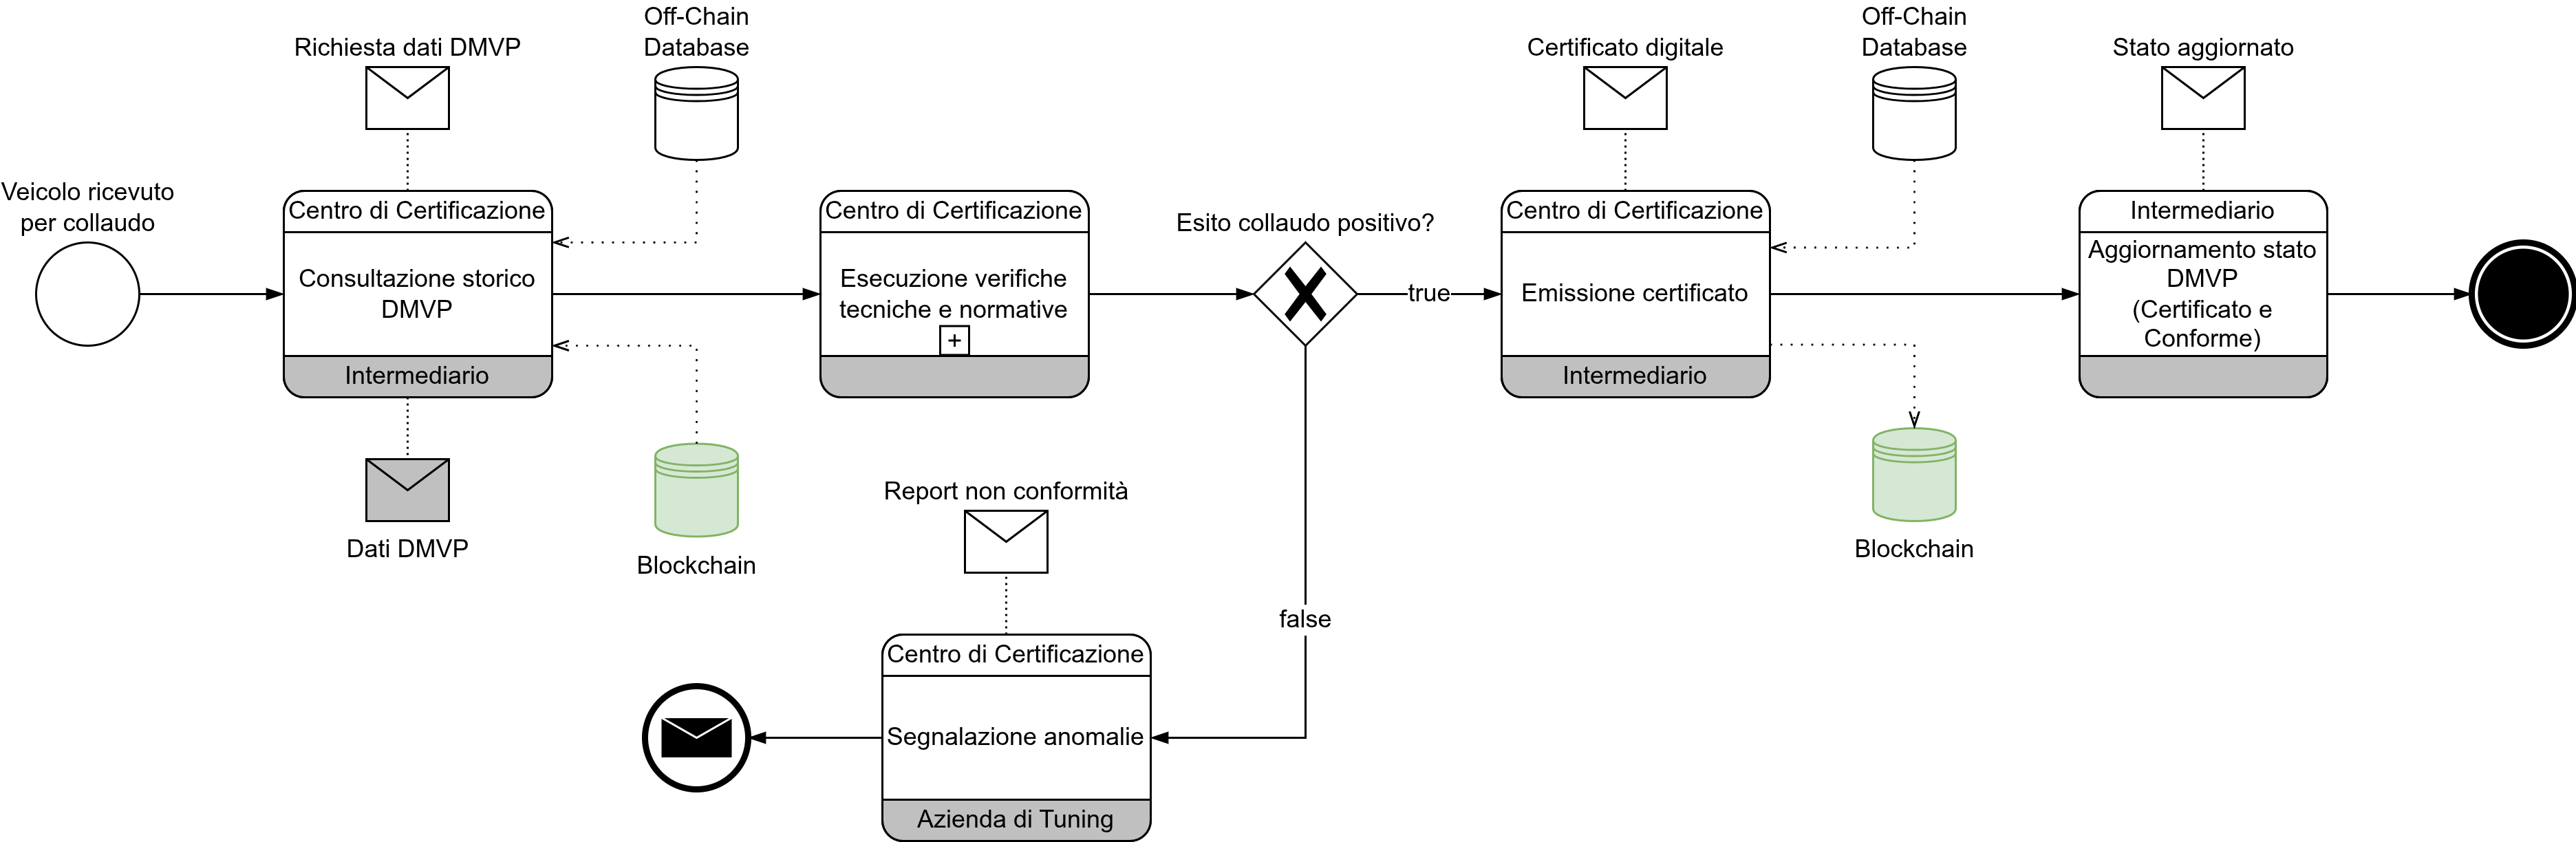
\includegraphics[width=\textwidth]{imgs/bpmn/03_ispezione_e_certificazione.png}
    \caption{Processo di ispezione e certificazione}
    \label{fig:bpmn-certificazione}
\end{figure}

\subsection*{Processo di Consegna del Veicolo e Trasferimento del DMVP}

L'ultimo processo (Figura~\ref{fig:bpmn-consegna}) modella la fase di consegna finale del veicolo e il trasferimento del passaporto digitale al Cliente Privato. Il flusso è avviato dalla Concessionaria a seguito della ricezione del veicolo omologato.

Il processo prevede la predisposizione del veicolo per la consegna finale, la consultazione dello storico del DMVP da parte del Cliente Privato --- che accede ai dati descrittivi conservati off-chain e ne verifica l'integrità sulla catena --- e infine l'accettazione formale del veicolo.

L'accettazione del cliente attiva l'operazione gestita dall'Intermediario attraverso la quale vengono trasferiti sulla blockchain i diritti di accesso e la proprietà del DMVP. L'evento finale segna la chiusura dell'intero ciclo di tracciabilità post-vendita del veicolo modificato.

\begin{figure}[H]
    \centering
    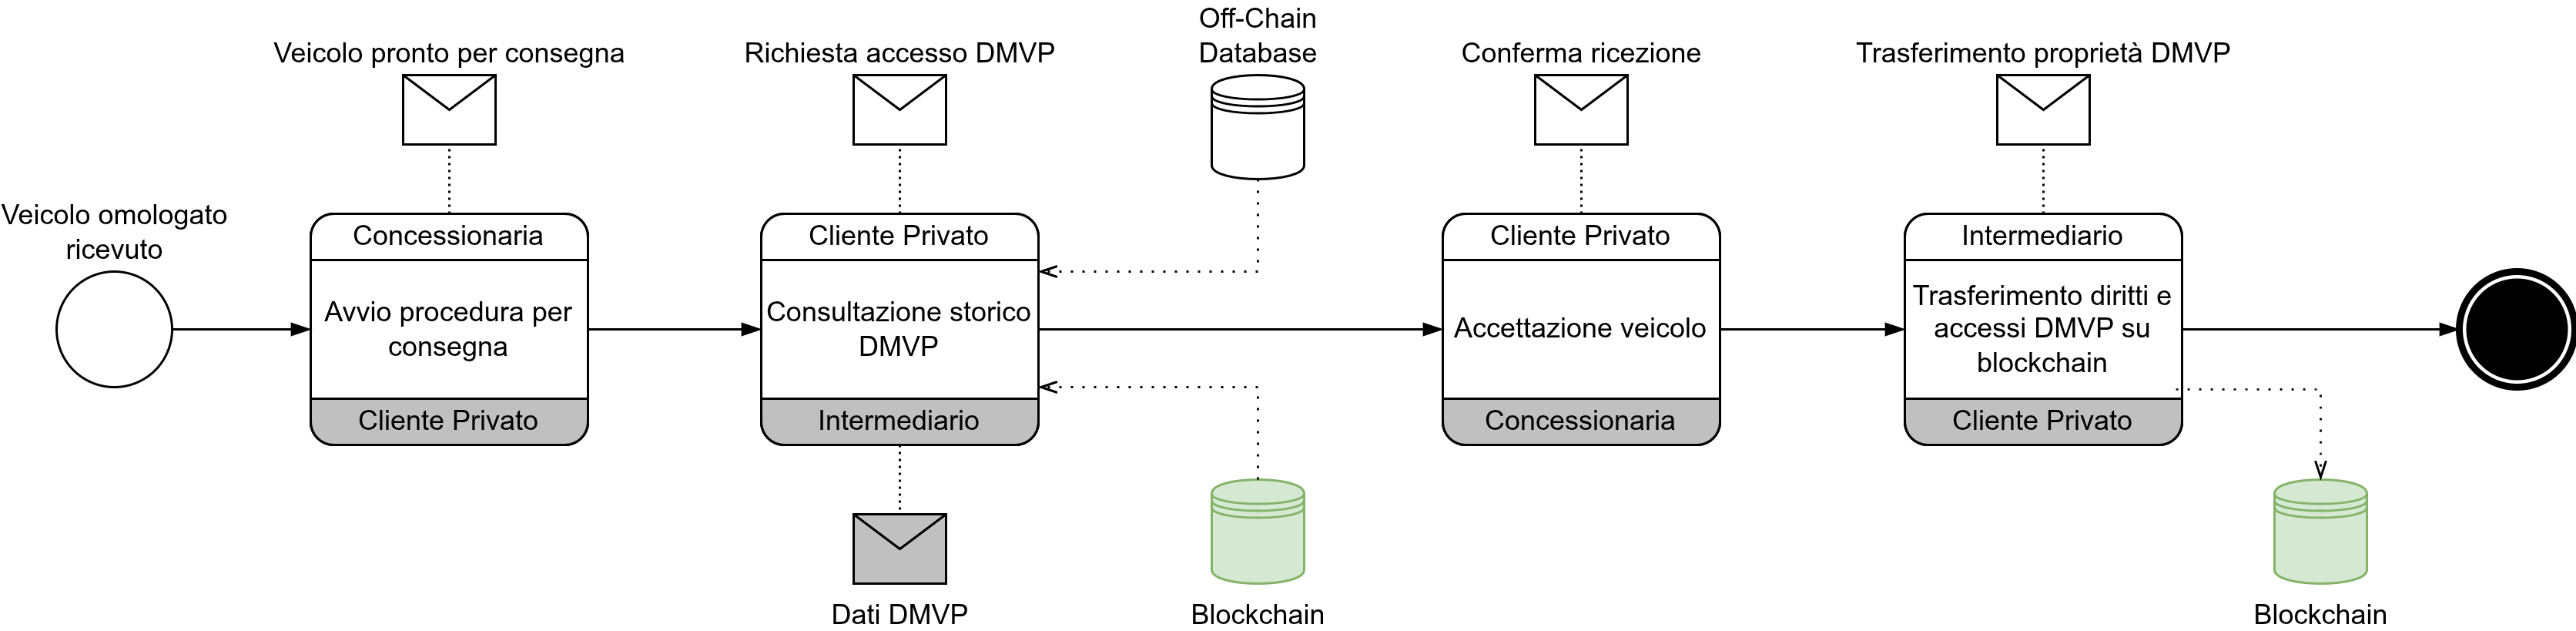
\includegraphics[width=\textwidth]{imgs/bpmn/04_consegna_veicolo_e_trasferimento_DMVP.png}
    \caption{Processo di consegna del veicolo e trasferimento del DMVP}
    \label{fig:bpmn-consegna}
\end{figure}